\documentclass[12pt,a4paper]{article}

\usepackage{amsmath,amsthm,amssymb}
\usepackage[utf8]{vietnam}
\usepackage{blindtext}
\usepackage{listings}
\usepackage[numbers]{natbib}
\usepackage{enumitem}
\usepackage{graphicx}
\usepackage{subcaption}
\captionsetup{compatibility=false}
\renewcommand{\baselinestretch}{1.5}
\begin{document}

%----------------------------------------------------------------------------------------
%	TITLE PAGE
%----------------------------------------------------------------------------------------

\begin{titlepage} % Suppresses displaying the page number on the title page and the subsequent page counts as page 1
	\newcommand{\HRule}{\rule{\linewidth}{0.5mm}} % Defines a new command for horizontal lines, change thickness here
	
	\center % Centre everything on the page
	
	%------------------------------------------------
	%	Headings
	%------------------------------------------------
	
	\textsc{\LARGE đại học khoa học tự nhiên}\\[1.5cm] 
	\textsc{\Large Khoa Toán-tin học}\\[0.5cm] 
	
	\textsc{\large Phương pháp toán trong tin}\\[0.5cm] 
	
	%------------------------------------------------
	%	Title
	%------------------------------------------------
	
	\HRule\\[0.4cm]
	
	{\huge\bfseries Exploiting reinforcement learning to find optimal strategy in dynamic maps}\\[0.4cm] % Title of your document
	
	\HRule\\[1.5cm]
	
	%------------------------------------------------
	%	Author(s)
	%------------------------------------------------
	
	\begin{minipage}{0.4\textwidth}
		\begin{flushleft}
			\large
			\textit{Tác giả}\\
			\textsc{Phan Quang Khánh} % Your name
		\end{flushleft}
	\end{minipage}
	~
	\begin{minipage}{0.4\textwidth}
		\begin{flushright}
			\large
			\textit{Giảng viên hướng dẫn}\\
			TS. Huỳnh Thế \textsc{Đăng} % Supervisor's name
		\end{flushright}
	\end{minipage}
	
	\vfill\vfill\vfill % Position the date 3/4 down the remaining page
	
	{\large\today} % Date, change the \today to a set date if you want to be precise
	
	%------------------------------------------------
	%	Logo
	%------------------------------------------------
	
	%\vfill\vfill
	%\includegraphics[width=0.2\textwidth]{placeholder.jpg}\\[1cm] % Include a department/university logo - this will require the graphicx package
	 
	%----------------------------------------------------------------------------------------
	
	\vfill % Push the date up 1/4 of the remaining page
	
\end{titlepage}
%---------------------------------------------------------------------------------
\clearpage
\tableofcontents
\clearpage
\section{Cơ sở lý thuyết}
\subsection{Q-learning}
Q-learning, trong đó đối tượng trong trò chơi\footnote{agent} tối ưu hàm phần thưởng đặc trưng của trò chơi bằng việc chọn hành động để tối đa hóa hàm tích lũy phần thưởng trong tương lai, là một trong những kỹ thuật mô hình hóa môi trường của agent và tập hành động của nó bằng quá trình quyết định Markov hữu hạn\footnote{finite Markov decision process}.\\
\subsection{SARSA}
\section{Quá trình}
\subsection{Lần thử thứ 1}
\subsubsection{Kết luận}
Agent không ra khỏi vùng an toàn, nghi ngờ rằng vì agent đi trên miền số nguyên mà enemy đi trên miền số thực dẫn đến việc khi tạo state cho model sẽ sinh ra rất nhiếu state. Do đó quá trình exploration của Q- learning sẽ trở nên nặng nề. 
\clearpage
\subsection{Lần thử thứ 2}
\subsubsection{Giả thiết}
Để khắc phục việc quá nhiều state, chúng tôi lấy phần nguyên của vị trí của enemy. Và để agent không ở lại trong vùng an toàn quá lâu, thay đổi trọng số của từng ô trong bản đồ là điều cần thiết.\\
Vì vùng an toàn quá lớn nên chúng tôi cắt giảm bớt bản đồ với kỳ vọng agent sẽ ra vùng nguy hiểm nhiều hơn..
\subsubsection{Thực hiện}
Với reward khi agent ở trên vùng an toàn sẽ bị trừ 1 mỗi lượt và khi trên vùng nguy hiểm sẽ được cộng 1.\\
Cắt giảm bản đồ khi giữ lại chỉ có 2 ô an toàn.\\
\begin{center}
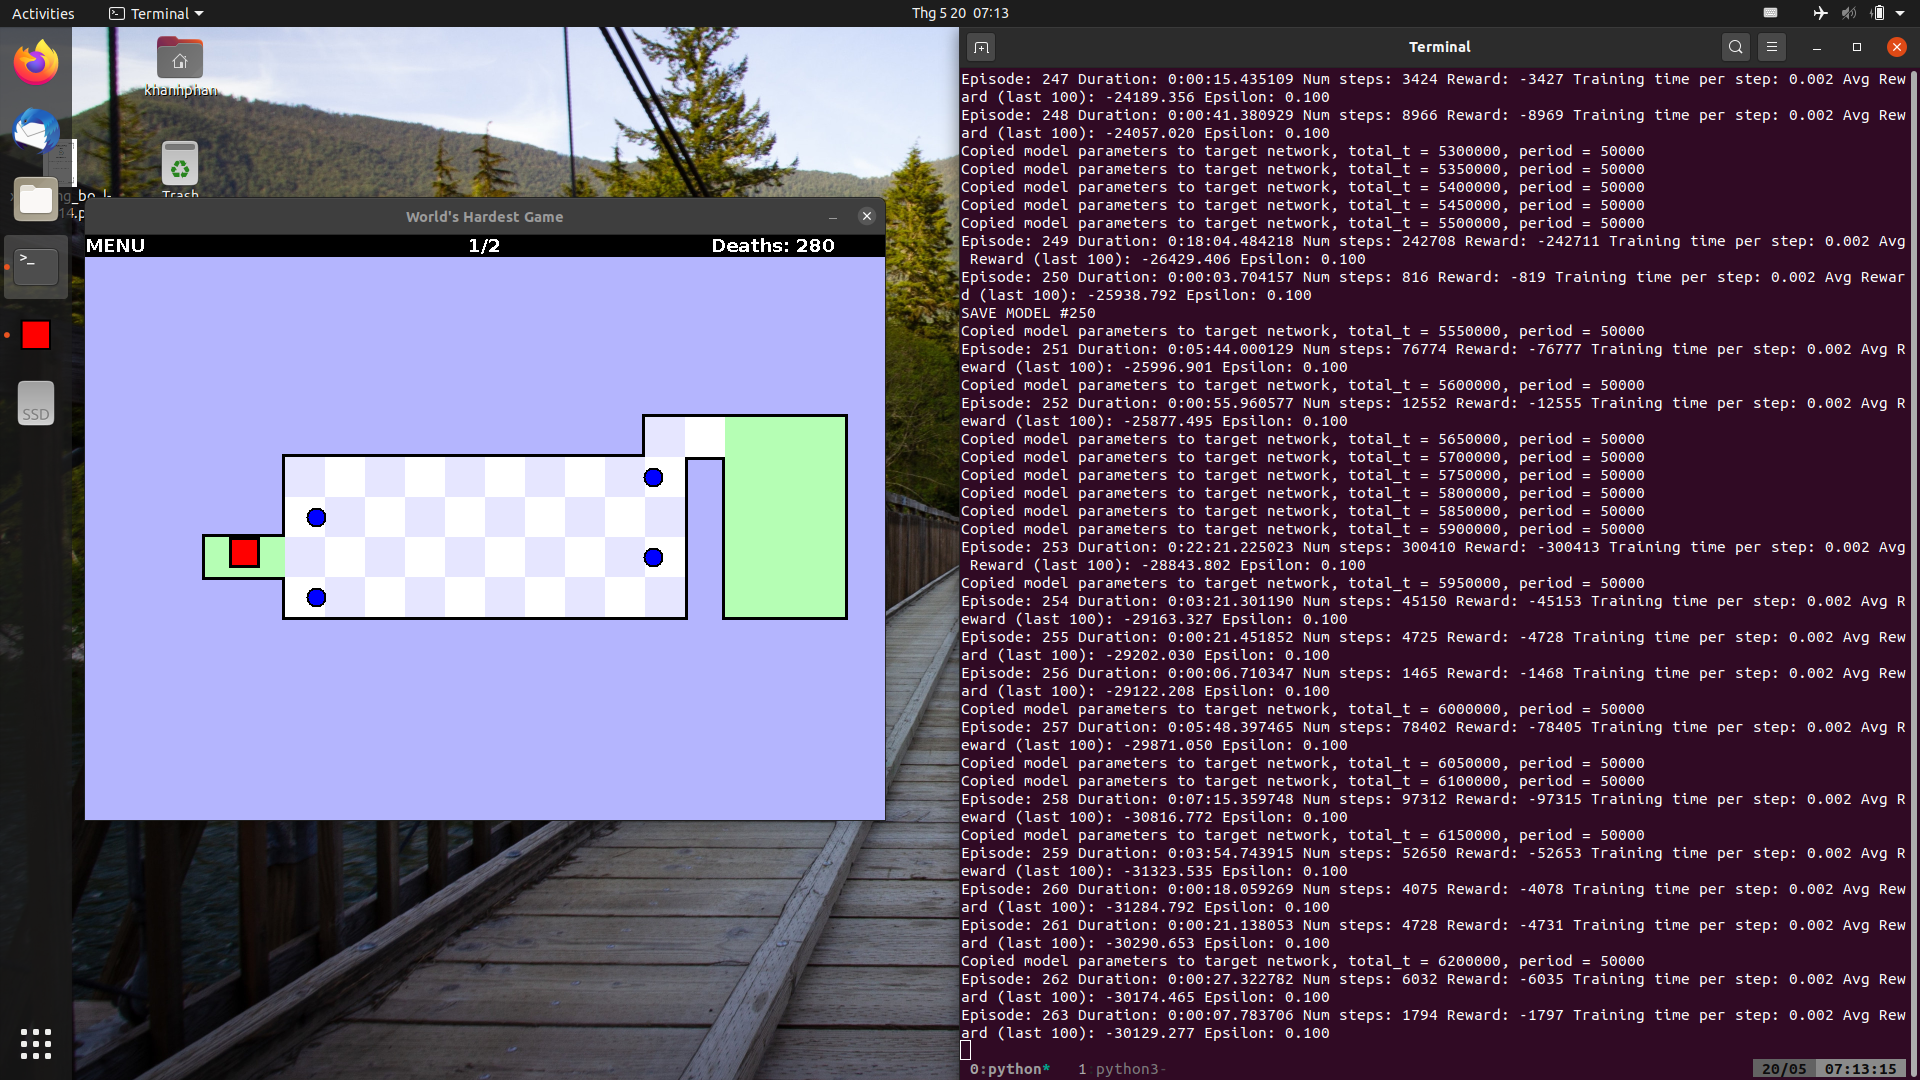
\includegraphics[width=0.95\textwidth]{Thesis_image/try2.png}\\    
\end{center}
Kết quả cho được không được như kỳ vọng sau khoảng 200 episodes, agent nhất quyết không ra khỏi vùng an toàn nữa.
\subsection{Môi trường đơn giản}
\subsubsection{1 Enemy}
Việc đơn giản hóa giúp điều chỉnh model hoạt động linh hoạt hơn\\
\begin{center}
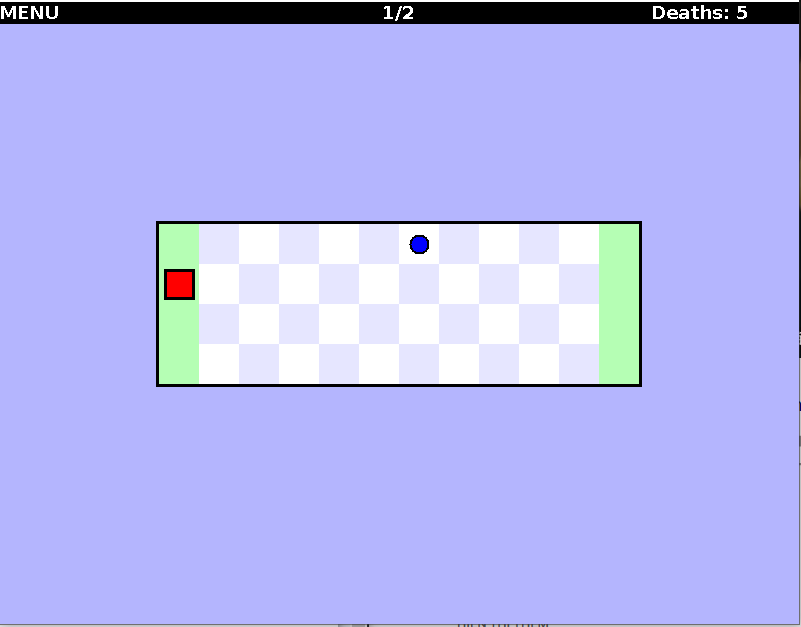
\includegraphics[width=0.5\textwidth]{photo/ThesisRES/1eUp.png}\\
\end{center}
Sử dụng với model gồm Q-learning gồm 2 layer (32 và 16), epsilon change\footnote{số lần thay đổi đổi tham số epsilon sau từng bước}(ES), số episode(eps). Các tham số còn lại sử dụng theo bài báo của deepmind.
\begin{figure}[h]
\centering
\begin{subfigure}[b]{.32\textwidth}
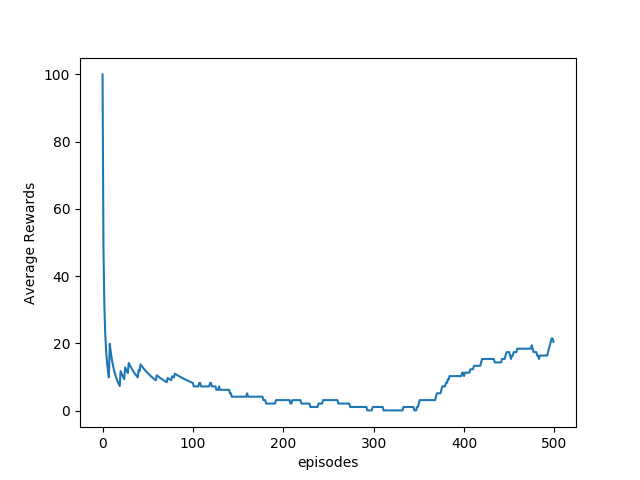
\includegraphics[width=0.9\linewidth, height=5cm]{pythonsection/result/result_1e_10000epsilon_500eps.png} 
\caption{10000 ES, 500 eps}
\label{fig:subim1}
\end{subfigure}
\begin{subfigure}[b]{.32\textwidth}
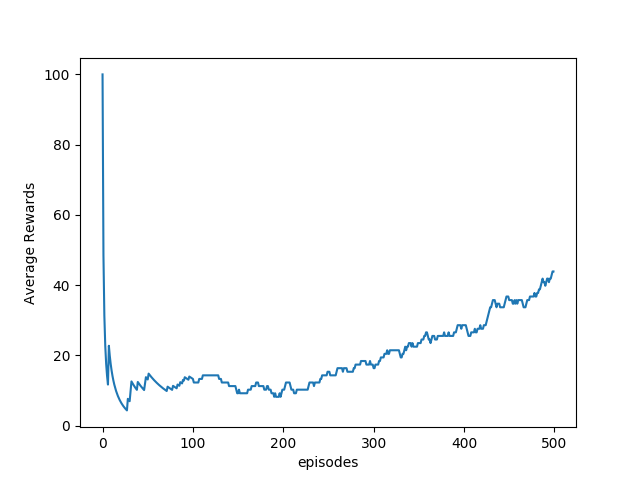
\includegraphics[width=0.9\linewidth, height=5cm]{pythonsection/result/result_1e_50000epsilon_500eps.png} 
\caption{50000 ES, 500 eps}
\label{fig:subim2}
\end{subfigure}
\begin{subfigure}[b]{.32\textwidth}
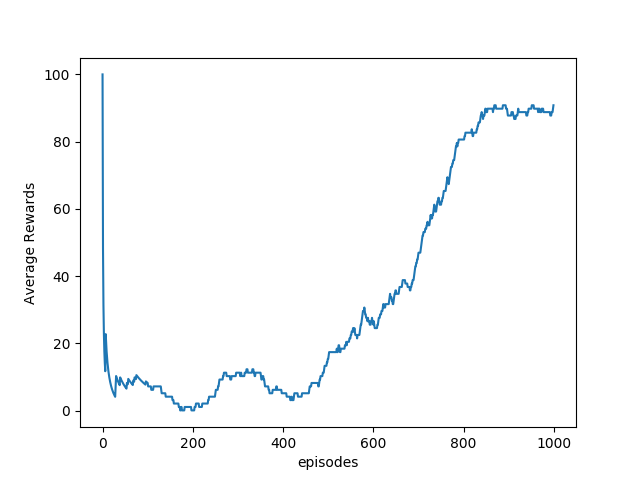
\includegraphics[width=0.9\linewidth, height=5cm]{pythonsection/result/result_1e_50000epsilon_1000eps.png} 
\caption{50000 ES và 1000 eps}
\label{fig:subim3}
\end{subfigure}
\end{figure}\\
Dựa vào kết quả trên có thể thấy sự ảnh hưởng của epsilon change và số lượng episode đối với kết quả của quá trình train là rất nhiều. Với hình (a) khi 
exploitation\footnote{agent thực hiện hành động tốt nhất} chiếm phần lớn thời gian agent hoạt động do đó quá trình huấn luyện không hiệu quả. Đối với hình (b) khi điểu chỉnh để exploration\footnote{agent thực hiện hành động ngẫu nhiên} và exploitation trở nên cân bằng hơn thì kết quả tốt hơn nhưng agent không đủ thời gian để đạt đến kết quả tốt nhất. Cuối cùng, kết quả có được ở hình (c) thể hiện agent hoạt động rất tốt.

\subsubsection{2 Enemy}
Áp dụng model ở trên cho môi trường có 2 enemy. Agent cần thêm 2000 episode để có thể tìm được đường đi tối ưu.\\
\begin{figure}[h]
    \centering
    \begin{subfigure}[b]{.32\textwidth}
    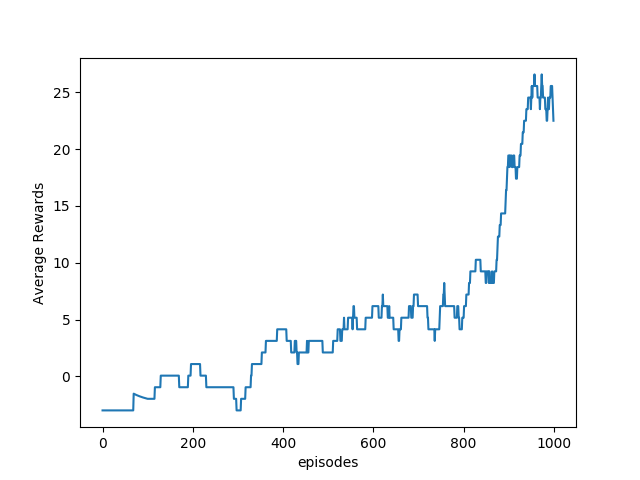
\includegraphics[width=0.9\linewidth, height=5cm]{pythonsection/result/result_2e_50000epsilon_1000eps.png}
    \caption{50000 ES và 1000 eps}
    \label{fig:2e1}
    \end{subfigure}
    \begin{subfigure}[b]{.32\textwidth}
    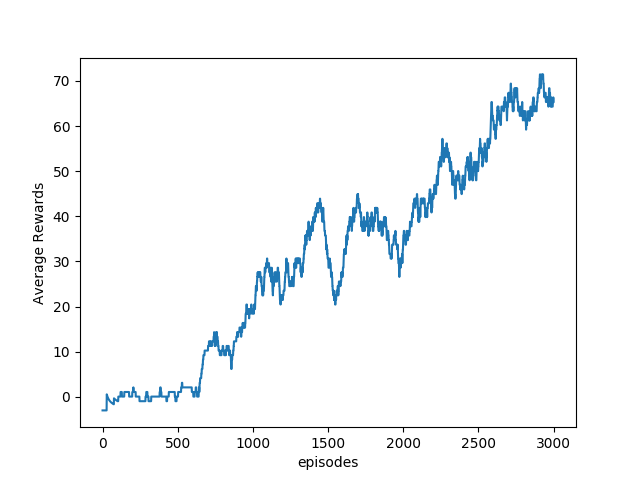
\includegraphics[width=0.9\linewidth, height=5cm]{pythonsection/result/result_2e_50000epsilon_3000eps.png}
    \caption{50000 ES và 3000 eps}
    \label{fig:2e2}
    \end{subfigure}
\end{figure}

\subsection{3 Enemy}
Dựa vào 2 kết quả trên có thể thấy khi agent có xu hướng tốt hơn trong các episode cuối cùng thì khi thêm số lần train sẽ cải thiện kết quả. Tuy nhiên với kết quả của trường hợp này lại không có xu hướng tăng. 
\end{document}